\chapter{Rezolucija}

\section{SAT problem}

U prošlom poglavlju definirali smo klauzule i klauzalne forme, i vidjeli kako se pomoću njih mogu zapisati proizvoljne formule. Svaka tautologija ekvivalentna je praznoj klauzalnoj formi, dok svaka oboriva formula ima svoju (jedinstvenu) savršenu klauzalnu formu kojoj je ekvivalentna. Dakle, klauzalne forme predstavljaju neku vrstu kanonskog oblika zapisa formule.

Vidjeli smo da je klauzalna forma valjana ako i samo ako su sve njene klauzule valjane (ovo naravno uključuje i slučaj kad je prazna), a valjane je klauzule lako prepoznati: samo mora postojati atom koji se nalazi i na lijevoj i na desnoj strani.

Drugim riječima, za klauzalnu formu postoji \emph{linearni} algoritam koji ustanovljuje je li valjana. Ovisno o implementaciji atoma i skupova taj algoritam može biti $O(n\log n)$ ili čak $O(n^2)$, ali u svakom slučaju je polinoman.

S druge strane, \emph{ispunjivost} klauzalne forme je puno teže ispitati. To je slavni SAT (\emph{satisfiability}) problem, prvi problem za kojeg je dokazano da je \emph{NP-potpun}. Više o tome čut ćete na kolegiju Složenost algoritama, ali ukratko, NP označava klasu problema za koje je u polinomnom vremenu ($p(n)$ koraka, gdje je $p$ neki polinom a $n$ broj bitova ulaza) moguće provjeriti je li zadani niz bitova (opet, veličine ograničene polinomom od $n$) validni \emph{certifikat} za rješenje.

Recimo, problem provjere je li zadani broj složen je u NP: faktorizacija može biti teška, ali ako nam netko dade faktor, lako je provjeriti da je ulaz njime djeljiv u polinomnom vremenu.

Svakako, sada vidimo da je SAT u NP: naći interpretaciju može biti teško, ali ako imamo interpretaciju, lako je u polinomnom  (precizno, kvadratnom) vremenu \emph{provjeriti} da je pod njom forma istinita. Zapravo vrijedi puno više od toga: ne samo da je SAT u NP, već se svaki problem $X$ u NP može \emph{svesti} na SAT: postoji polinomni algoritam koji preslikava instance problema $X$ u instance problema SAT (to su klauzalne forme), čuvajući rješivost: zadana instanca problema $X$ ima rješenje ako i samo ako je odgovarajuća klauzalna forma ispunjiva.

Iz toga slijedi da, kad bismo imali polinomni algoritam za rješavanje problema SAT, zapravo bismo imali polinomni algoritam za rješavanje \emph{svih} problema u NP, odnosno vrijedilo bi $P=NP$ ($P$ označava klasu problema za čije rješavanje postoji polinomni algoritam).
Mnogi stručnjaci za složenost u to sumnjaju, a za matematički dokaz točnog odnosa između $P$ i $NP$ Clay Institute nudi milijun dolara još od 2000.\ godine.

Iako mnogi vjeruju da svaki algoritam za SAT problem ima puno slu\-ča\-je\-va u kojima nema bitno boljeg rješenja od jednostavnog eksponencijalnog ispitivanja svih $2^n$ mogućnosti (gdje je $n$ broj različitih atoma koji se pojavljuju u klauzalnoj formi), ipak postoje mnoge heuristike, koje dodatno dobivaju na značenju činjenicom da su mnogi vrlo stvarni problemi (primjerice, problem rasporeda sati) u NP, pa se mogu izraziti kao instance SAT problema.

Ne sve, ali mnoge od tih heuristika zasnivaju se na \emph{rezoluciji}, jednostavnom logičkom principu koji nam omogućuje da od dvije klauzule dobijemo jednu novu, koju onda možemo koristiti dalje. No prvo pogledajmo neke slučajeve koje možemo riješiti jednustavnijim heuristikama.

\section{Jednostavni slučajevi i DPLL algoritam}

Iako moramo samo odrediti je li forma ispunjiva (da/ne), za dalja raz\-miš\-lja\-nja pomoći će ako se ponašamo kao da moramo baš naći interpretaciju $I_1$ koja je čini istinitom.

Prvo, očito atome koji se uopće ne pojavljuju možemo ignorirati, odnosno interpretaciju $I_1$ ne moramo definirati na njima. Što je s atomima koji se pojavljuju samo jednom? Lako je vidjeti da ih možemo iskoristiti kao ``džokere'': ako se pojavljuju na lijevoj strani klauzule, definiramo $I_1$ na njima kao $1$, a ako se pojavljuju na desnoj, definiramo $I_1$ na njima kao $0$.

Ta klauzula time postaje zadovoljena i možemo je brisati iz klauzalne forme. Štoviše, sad se lako vidi da potpuno isti pristup funkcionira i ako se određeni atom pojavljuje više puta, ali uvijek na istoj strani klauzule (uvijek na lijevoj, ili uvijek na desnoj). Takvi atomi zovu se \emph{čisti} atomi.

Idemo dalje. Što ako se neki atom pojavljuje dvaput, na različitim stranama klauzule? Ako se pojavljuje na različitim stranama \emph{iste} klauzule, tad znamo da je ta klauzula tautologija, pa je uvijek zadovoljena i možemo je brisati. Netrivijalan slučaj nastupa ako se isti atom pojavljuje na različitim stranama dviju različitih klauzula, i razmatranje tog slučaja vodi na rezoluciju. Zasad samo pogledajmo još nekoliko jednostavnih slučajeva.

Ako se neka (\enquote{jedinična}) klauzula sastoji samo od jednog atoma $p$, vrijednost $I_1(p)$ je time fiksirana: ako imamo klauzulu $p\leftarrow$, mora biti $I_1(p)=1$, a ako imamo klauzulu $\leftarrow p$, mora biti $I_1(p)=0$. Time ne samo da je ta klauzula zadovoljena, već možemo brisati $p$ iz svih ostalih klauzula u kojima se pojavljuje. Ako se pojavljuje na istoj strani kao u jediničnoj klauzuli, možemo obrisati i čitavu tu klauzulu, jer znamo da je ispunjena. Ako je na suprotnoj strani nego u jediničnoj klauzuli, možemo samo brisati taj atom, ali time i ta klauzula može postati jedinična, te se postupak može nastaviti dalje.

Zapažanje iz prethodnog odlomka možemo generalizirati na još jedan način: za klauzulu $A\leftarrow B$ kažemo da \emph{obuhvaća} klauzulu $C\leftarrow D$ ako je $A\subseteq C\land B\subseteq D$. Lako je vidjeti da u tom slučaju bilo koja interpretacija pod kojom je istinita $A\leftarrow B$, čini istinitom i klauzulu $C\leftarrow D$ --- odnosno, ako je $A\leftarrow B$ element naše klauzalne forme čiju ispunjivost ispitujemo, tada možemo iz nje brisati sve klauzule $C\leftarrow D$ koje su njome obuhvaćene.

Sistematska razrada upravo opisanih ideja vodi na DPLL, vjerojatno najpoznatiji \enquote{generički} algoritam za rješavanje SAT problema. Na profinjenjima toga algoritma radi se i danas, prvenstveno u tri smjera:
\begin{enumerate}
	\item Ako ne nastupa nijedan od gore navedenih specijalnih slučajeva, moramo pametno odabrati neki atom, te vrijednost koju ćemo mu pokušati pridružiti. Naravno, ako ta grana ne uspije, moramo se vratiti (\emph{backtrack}) i pokušati mu pridružiti suprotnu vrijednost. Strategijâ za odabir ima puno, vrlo je netrivijalno naći pravu, a bitno utječu na kasnije odvijanje algoritma i veličinu preostalog prostora mogućnosti koje treba ispitati.
	\item Eliminacija atoma koji se pojavljuju u jediničnim klauzulama, rekli smo, može dovesti do stvaranja novih jediničnih klauzula, što može stvoriti duge \enquote{domino-lance} klauzulâ. Netrivijalno je smisliti dobru strukturu podataka koja će takvu operaciju izvršavati vrlo brzo, pogotovo uzevši u obzir da i vraćanje prethodnog stanja mora biti brzo zbog čestog \emph{backtracking}a.
	\item U zadnjem desetljeću naučili smo mnoge nove trikove vezane uz strojno učenje. Vrlo je plodno područje pokušaja implementacije tih trikova u DPLL algoritmu. Recimo, jedna od mogućnosti je natjerati algoritam da uoči ako mu se neki \emph{cluster} u $I_1$ uvijek iznova pokaže proturječnim, te ga počne izbjegavati (odnosno prije njegovog ispitivanja pokušati nešto drugo) u kasnijim grananjima.
\end{enumerate}

\section{Rezolucija}

Jednostavna analogija koja nam može pomoći razumjeti ideju rezolucije je sljedeća: zamislimo da ispred sebe imamo puno klauzula, i moramo naći vrijednosti koje ćemo pridružiti atomima tako da sve one budu istinite. Kad ga gledamo na taj način, problem donekle podsjeća na rješavanje sustava jednadžbi: svaka može biti zadovoljena na razne načine jer ima puno nepoznanica, ali uvjet da \emph{sve} moraju biti zadovoljene bitno smanjuje broj mogućnosti.

Tehnika koju obično koristimo kod rješavanja sustava algebarskih jednadžbi je \emph{supstitucija}. Njome iz para jednadžbi eliminiramo jednu nepoznanicu, tako da je izrazimo iz jedne i uvrstimo izraz za nju u onu drugu. Zapravo, često ako su jednadžbe dovoljno pravilne strukture, i ne moramo izražavati pa uvrštavati: jednostavnim agregiranjem (zbrajanjem) jednadžbi kojima se nepoznanica nalazi na suprotnim stranama, ona se reducira (po\-ni\-šta\-va) i time nestaje iz rezultatne jednadžbe.
$$\left.\begin{array}{r@{\;=\;}l}x+\cancel{y}&a+b\\c&\cancel{y}+z\end{array}\right\}\quad\Longrightarrow\quad x + c = a + b + z$$
Klauzule \emph{jesu} vrlo pravilne strukture (iako nesimetričnost znači da bolje odgovaraju \emph{nejednadžbama} nego jednadžbama), i pokazuje se da je vrlo sličan manevar moguće napraviti s njima. 

Dakle, rezoluciju primjenjujemo kad imamo isti atom na različitim stranama dvije klauzule. Takve klauzule zovemo \emph{ulančanima}. Precizno, klauzule $A\leftarrow B$ i $C\leftarrow D$ su ulančane ako je $(A\cap D)\cup(B\cap C)\not=\emptyset$. Odaberimo jedan element tog presjeka, neka je to $q$. (Poslije ćemo vidjeti da je zapravo jedini zanimljiv slučaj kad je $q$ jedinstven.) Bez smanjenja općenitosti (inače zamijenimo klauzule), $q\in A\cap D$. Vrijednost $I_1(q)$ je ili $0$ ili $1$. Ako je $0$, klauzula $C\leftarrow D$ je istinita (jer je $q\in D$), i trebamo samo gledati $A\setminus\{q\}\leftarrow B$. Ako je pak $1$, klauzula $A\leftarrow B$ je istinita (jer je $q\in A$), i trebamo samo gledati $C\leftarrow D\setminus\{q\}$.

Dakle, ako je $I_1$ rješenje, tada je ili neki atom iz $A\setminus\{q\}$ istinit, ili je neki atom iz $B$ lažan, ili je neki atom iz $C$ istinit, ili je neki atom iz $D\setminus\{q\}$ lažan. Pišući to drugim redom (grupirajući posebno istinite a posebno lažne mogućnosti), dobivamo da je pod $I_1$ istinita klauzula $$(A\setminus\{q\})\cup C\leftarrow B\cup(D\setminus\{q\})\;,$$
koju zovemo \emph{rezolventom} klauzula $A\leftarrow B$ i $C\leftarrow D$, i označavamo je oznakom $(C\leftarrow D)\;\cancel{q}\;(A\leftarrow B)$. Proces kojim je ta klauzula dobivena od početnih zovemo \emph{rezolucijom}.

Vidjeli smo da ako su dvije klauzule ulančane i istinite pod nekom interpretacijom, tada je pod istom interpretacijom istinita i njihova rezolventa s obzirom na neki atom po kojem su ulančane. Što ako ima više takvih atoma? Lako je vidjeti da ako su različiti atomi $q$ i $r$ svaki na različitim stranama dvije klauzule, tada ako napravimo rezoluciju po $q$, rezolventa će imati $r$ na obje strane, i jednako tako ako napravimo rezoluciju po $r$, rezolventa će imati $q$ na obje strane. U svakom slučaju rezolventa će biti tautologija, pa je možemo brisati iz klauzalne forme. Iz tog razloga rezolventa se obično gleda samo kad imamo jedinstveni atom na suprotnim stranama dvije različite klauzule.

Opet, jasno je da se postupak može provesti i ako se $q$ javlja na više od dva mjesta, u ostalim klauzulama. Tada nismo eliminirali nepoznanicu u potpunosti, ali smo svejedno napravili korak prema pojednostavljenju.

Nažalost, kao i u slučaju rješavanja linearnih sustava, ne možemo rezolvirane klauzule jednostavno zamijeniti rezolventom, već moramo rezolventu dodati u skup klauzula koje razmatramo. Ipak, taj postupak će za konačne klauzalne forme stati iz jednostavnog razloga što u početku imamo samo konačno mnogo atoma, rezolucija ne stvara nove atome, a \emph{svih} klauzula nad konačno mnogo atoma ima samo konačno mnogo.

\begin{zadatak}-
	Dokažite da svih relevantnih (ispunjivih i oborivih) klauzula nad $n$ atoma ima $3^n-1$.
\end{zadatak}

Dakle, algoritam rezolucije je sljedeći:

\begin{algorithmic}
	\Require $S$ je konačna klauzalna forma (skup klauzula).
	\ForAll {klauzule $(A\leftarrow B), (C\leftarrow D)\in S$}
		\If {$\left|A\cap D\right|=1 \And B\cap C=\emptyset$}
			\State $q:=\mbox{jedini element od }A\cap D$
			\State $\mbox{rezolventa}:=(A\setminus\{q\})\cup C\leftarrow B\cup(D\setminus\{q\})$
			\If {rezolventa = $(\leftarrow)$}
				\Return \enquote{$S$ je proturječna!}
			\EndIf
			\State $S:=S\cup \{\mbox{rezolventa}\}$
		\EndIf
	\EndFor
\end{algorithmic}

Sasvim je jasno iz prethodnih razmatranja (ako su dvije ulančane klauzule istinite pod $I_1$, tada je i njihova rezolventa istinita pod istom interpretacijom) da algoritam rezolucije pokrenut na ispunjivoj klauzalnoj formi $S$ može generirati samo ispunjive rezolvente, pa nikada ne može javiti da je $S$ proturječna. To znači da je algoritam rezolucije \emph{adekvatan} za logiku sudova.

\section{Potpunost algoritma rezolucije}

Zapravo vrijedi i obrat: algoritam rezolucije je i \emph{potpun} za logiku sudova, što znači da ako je početna klauzalna forma proturječna, algoritam ne može ispitati \emph{sve} parove klauzula (uključujući novododane klauzule) a da ne generira praznu klauzulu. Štoviše, jer svih klauzula koje algoritam rezolucije može generirati ima konačno mnogo, algoritam će sigurno stati, i adekvatnost i potpunost tada znače da će dati točan rezultat: \enquote{$S$ je proturječna} ako i samo ako $S$ doista jest proturječna.

Precizan dokaz potpunosti može se naći u~\cite{BenAri} i predstavlja dobru temu za seminar. Ovdje samo dajemo ideju dokaza.

Poredajmo atome u $S$ u kanonskom redoslijedu (slova po abecedi, neindeksirani prije indeksiranih, indeksirani atomi istog slova po indeksu) i nazovimo ih $a_1$, $a_2$, \ldots, $a_n$. Za $1\le k\le n$, $k$-klauzulom zovemo oborivu klauzulu $A\leftarrow B$ čiji je $Var$ skup prvih $k$ atoma $\{a_1,...a_k\}$.
Sada promotrimo potpuno binarno stablo visine $n$ na čijoj $k$-toj razini se nalaze upravo sve $k$-klauzule (njih $2^k$), te su djeca (za $k<n$) svake takve klauzule
$A\leftarrow B$ dvije klauzule koje nastaju dodavanjem atoma $a_{k+1}$ na svaku stranu ($A\cup\{a_{k+1}\}\leftarrow B$ lijevo, $A\leftarrow B\cup\{a_{k+1}\}$ desno). 

Dakle, u korijenu je prazna klauzula: jedina $0$-klauzula. Također primijetimo da u svakom putu u stablu, gornja klauzula obuhvaća donju. Za kraj još primijetimo da je svaki unutarnji čvor upravo rezolventa svoje djece: $$(A\cup\{a_{k+1}\}\leftarrow B)\;\cancel{a_{k+1}}\;(A\leftarrow B\cup\{a_{k+1}\})=A\leftarrow B\;.$$
Neke od tih $2^{n+1}-1$ klauzula su u $S$, ali moguće je da u $S$ imamo i klauzule koje nisu u stablu (npr.\ $a_3\leftarrow a_1$). Ipak, za svaku klauzulu $K\in S$ ima bar jedna (među listovima njih točno $2^{n-\left|Vars(K)\right|}$) klauzula koju $K$ obuhvaća.

Ako sada u stablu \enquote{blokiramo} sve klauzule obuhvaćene elementima iz $S$, lako se vidi da proturječnost od $S$ znači da je svaki put od korijena do lista negdje blokiran. Naime, dualno, putovi od korijena do lista odgovaraju interpretacijama za $S$, pri čemu izbor smjera kojim treba ići na $k$.\ razini odgovara vrijednosti interpretacije na $a_k$ (lijevo znači $I(a_k)=0$, desno znači $I(a_k)=1$). Lako se vidi da takva interpretacija čini lažnima samo klauzule do kojih njen put dolazi. Kad neki put ne bi bio blokiran, interpretacija njime određena bi činila istinitom čitav $S$.

Blokirane klauzule ne moraju dakle nužno biti doista elementi od $S$, ali možemo se pretvarati kao da jesu: obuhvaćene su njima, pa će rezolucija na blokiranim klauzulama dati klauzulu koja je obuhvaćena rezolventom neke dvije klauzule koje doista jesu u $S$. (Ovo je najmutniji dio, zbog kojeg je ovo samo ideja dokaza. Trebalo bi pokazati da rezolucija čuva relaciju uređaja po obuhvaćenosti.)

\begin{tikzpicture}
\Tree 
[.$\leftarrow$
 [.$p\leftarrow$
  [.$p,q\leftarrow$
    [.{\scriptsize $p,q,r\leftarrow$} ]
    [.{\scriptsize $p,q\leftarrow r$} ]
  ]
  [.$p\leftarrow q$
  	[.{\scriptsize
  		$p,r\leftarrow q$} ]
  	[.{\scriptsize
  		$p\leftarrow q,r$} ]
  ]
 ]
 [.$\leftarrow p$
  [.$q\leftarrow p$
    [.{\scriptsize
    	$q,r\leftarrow p$} ]
    [.{\scriptsize
    	$q\leftarrow p,r$} ]
  ]
  [.$\leftarrow p,q$
  	[.{\scriptsize
  		$r\leftarrow p,q$} ]
  	[.{\scriptsize
  		$\leftarrow p,q,r$} ]
  ]
 ]
]

\end{tikzpicture}

Sada je ključno primijetiti da svako takvo \enquote{blokiranje} mora ili imati blokiran korijen (u kom slučaju smo gotovi, jer je prazna klauzula element od $S$), ili imati neblokiran unutarnji čvor čija oba djeteta su blokirana. Primjerice, bilo koji neblokirani čvor maksimalne udaljenosti do korijena mora imati to svojstvo.

No vidjeli smo da je svaki čvor, pa tako i taj, rezolventa svoje djece. Kako su mu djeca blokirana, rezolucijom možemo dobiti njega, obuhvaćenog nekom rezolventom elemenata iz $S$. To znači da i taj čvor možemo blokirati. Sada smo dobili novo stablo, iste strukture kao prije, samo s jednim blokiranim čvorom više.

Kako je i s tim stablom moguće ponoviti isti postupak, i tako u nedogled, a svih čvorova ima konačno mnogo, postupak će prije ili kasnije završiti, a jedino može završiti blokiranjem korijena. To bi značilo da je prazna klauzula obuhvaćena nekim elementom koji je došao u $S$ --- no prazna klauzula može biti obuhvaćena jedino samom sobom, dakle prazna klauzula je u nekom trenutku došla u $S$.

Kako algoritam rezolucije ispituje parove klauzula nekim redom, prije ili kasnije će naići upravo na par koji smo razmatrali ovdje, te će nakon toga u nekom trenutku \enquote{nabasati} na pravi par za dalje smanjenje, i tako dalje. Dakle, nakon dovoljno mnogo vremena, algoritam rezolucije pokrenut na proturječnoj klauzalnoj formi otkrit će da je proturječna (možda vrlo brzo, ako mu se \enquote{posreći}, a možda vrlo sporo, ali svakako u konačno mnogo koraka).

Jednako tako, ispunjivost klauzalne forme znači postojanje bar jednog puta od korijena do lista koji nije blokiran. Tada ako označimo sve takve putove, lako se vidi da primjena rezolucije nikada ne može blokirati nijedan čvor na takvim putovima. Kad označi sve ostale čvorove, algoritam rezolucije će stati, te ćemo znati da forma nije proturječna.

Takvo stablo, tzv.\ semantičko stablo, pruža dobar uvid i u ideju dokaza teorema kompaktnosti za logiku sudova: čak i ako je stablo beskonačno u visinu, svejedno će svaka staza od korijena prije ili kasnije biti blokirana, ili će postojati beskonačni put od korijena prema dolje, što će generirati interpretaciju.